\documentclass[11pt, oneside]{article} 
\usepackage{geometry}
\geometry{letterpaper} 
\usepackage{graphicx}
	
\usepackage{amssymb}
\usepackage{amsmath}
\usepackage{parskip}
\usepackage{color}
\usepackage{hyperref}

\graphicspath{{/Users/telliott/Github/calculus_book/png/}}
% \begin{center} \includegraphics [scale=0.4] {gauss3.png} \end{center}

\title{Archimedes and pi}
\date{}

\begin{document}
\maketitle
\Large

\label{sec:Archimedes_and_pi}

We're going to follow a page that in turn follows Archimedes argument for the approximation of $\pi$.

\url{https://itech.fgcu.edu/faculty/clindsey/mhf4404/archimedes/archimedes.html}

Before we start, let's review some ideas related to angle bisection.  Recall that if we have an angle bisector in a right triangle (left panel), the theorem says that 
\[ \frac{a}{c} = \frac{b}{d} \]
\begin{center} 
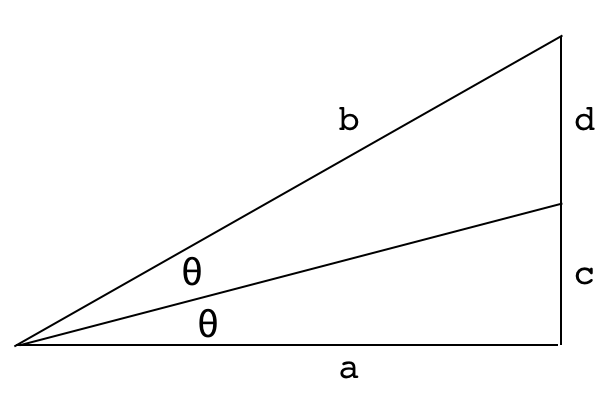
\includegraphics [scale=0.3] {pi3.png} 
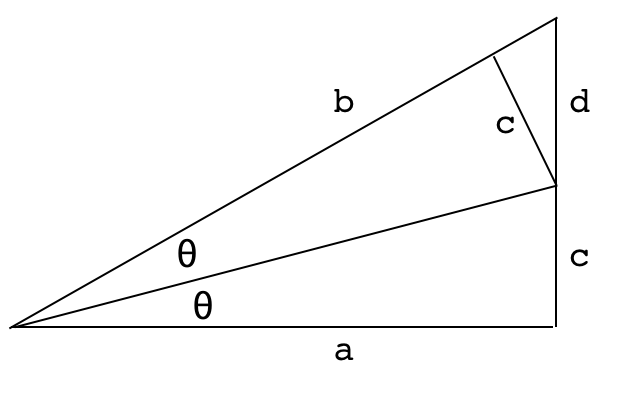
\includegraphics [scale=0.3] {pi4.png} 
\end{center}
The proof (which we showed in an earlier chapter) involves drawing the altitude of the top triangle, forming two congruent triangles and a smaller one which is easily shown to be similar to the original triangle (right panel).  By similar triangles, we have 
\[ \frac{d}{c} = \frac{b}{a} \]
which can be rearranged to give the desired statement.  A corollary follows:
\[ \frac{a}{b} = \frac{c}{d} \]
\[ \frac{a + b}{b} = \frac{c + d}{d} \]
\[ \frac{a + b}{c + d} = \frac{b}{d} = \frac{a}{c} \]
\begin{center} 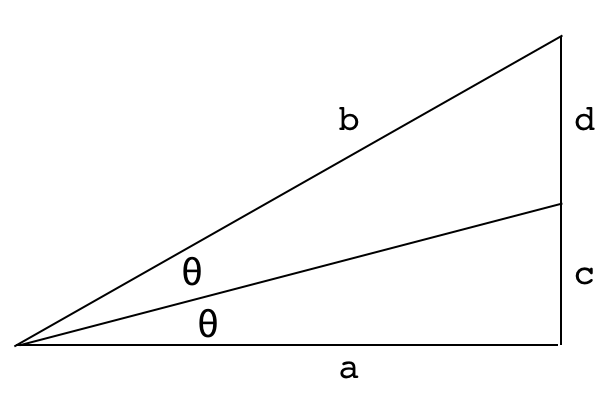
\includegraphics [scale=0.3] {pi3.png} \end{center}
This doesn't seem obvious to me, in fact it seems counter-intuitive.  Nonetheless, we will use it extensively for what follows.

 \subsection*{overview}
 There are three steps which we will repeat (eventually, four times).  
 
 Let's relabel the figure now:
 \begin{center} 
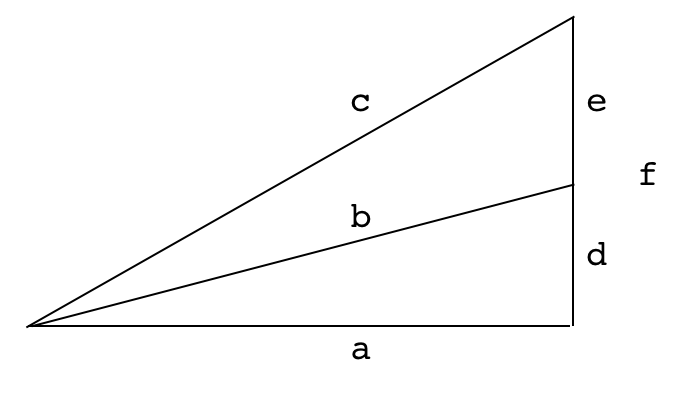
\includegraphics [scale=0.3] {pi6.png} 
\end{center}

 $\bullet$ Obtain ratios for the cosecant and cotangent ($c/f$ and $a/f$).  In the first round, these are just $\sqrt{3}$ and $2$.
 
 $\bullet$ Add them together, obtaining $(c + a)/f$ and observe that this ratio is also equal to $a/d$, by the corollary of the angle bisector theorem above.  This gives us the cotangent of the half-angle.
 
 $\bullet$ Obtain the cosecant of the half-angle, $b/d$, by using the Pythagorean theorem.  Namely:
 \[ a^2 + d^2 = b^2 \]
\[ \sqrt{\frac{a^2}{d^2} + 1} = \frac{b}{d} \]

\subsection*{Part A, round 1}
Draw a circle with radius $OA$ and tangent $AC$, and let $\angle AOC$ be one-third of a right angle.
\begin{center} 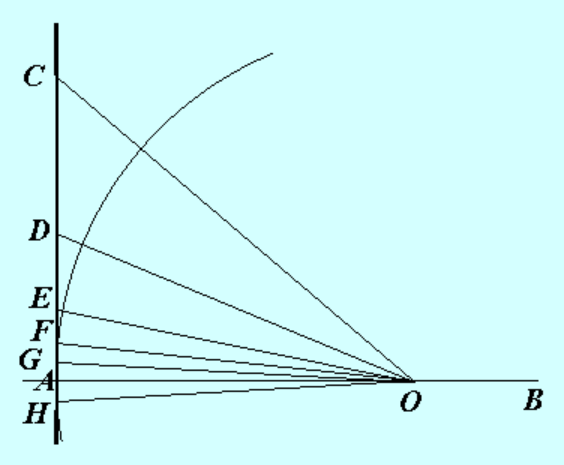
\includegraphics [scale=0.3] {pi5.png} \end{center}

Note: the figure appears to have been compressed in width.  The angle bisectors don't look right and the original angle looks more like $45$ than $30$.  We'll use it anyway.

In what follows we list the claim first:

$\bullet$   $OA:AC > 265:153$

Followed by the proof:

Since the triangle is a 30-60-90 triangle, $OA = \sqrt{3}$ and $AC = 1$, so the ratio is just $\sqrt{3}$.  $265/153$ is a (very good) approximation, just slightly smaller than the true value.

$\bullet$   $OC:AC = 306:153$

The cosecant $= 2$.  The denominator has been chosen to match the previous ratio.  

Now draw the angle bisector $OD$.

$\bullet$   $CO : OA = CD : DA$

This is just the angle bisector theorem.
\begin{center} 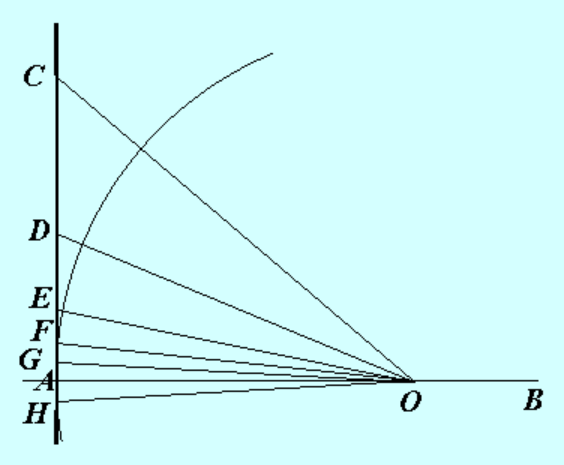
\includegraphics [scale=0.3] {pi5.png} \end{center}
$\bullet$   $(CO + OA) : CA = OA : AD$

This ratio is equal to that from the bisector theorem by the corollary.  Start with
\[ CO:OA = CD:DA \]
\[ \frac{CO + OA}{OA} = \frac{CD + DA}{DA} = \frac{CA}{DA} \]

This crucial step gives us the cotangent of the half-angle formed by the angle bisector $OD$.

$\bullet$   $OA : AD > 571 : 153$

We just add numerators for the first two ratios above, leaving the result over the common denominator.

$\bullet$   $OD : AD > 591\ 1/8 : 153$

Finally, we want $OD : AD$.  By the Pythagorean Theorem
\[ OD^2 = OA^2 + AD^2 \]
\[ (OD : AD)^2 = (OA : AD)^2 + 1 \]

Now do $571^2 = 326041;  153^2 = 23409$ so the sum of numerators is $349450$ and the square root is $591 \ 1/6$.

Archimedes approximates the result as 591\ 1/8 : 153.  Remember that we are looking for a lower bound,  so smaller is OK.

\subsection*{Part A, round 2}

Now draw the angle bisector $OE$.

\begin{center} 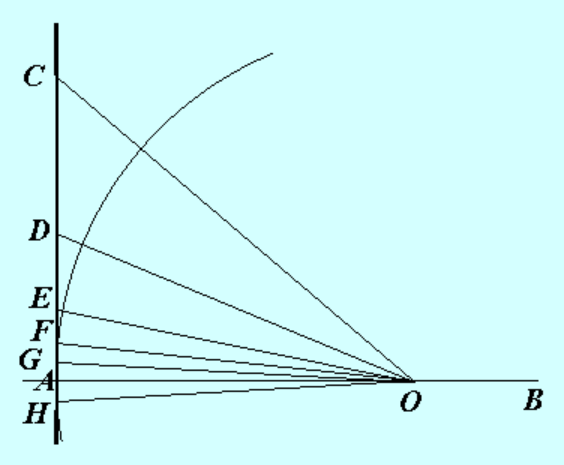
\includegraphics [scale=0.3] {pi5.png} \end{center}

$\bullet$ From above, we have that $OA : AD > 571 : 153$ and $OD : AD > 591\ 1/8 : 153$.

$\bullet$   $OA : AE > 1162\ 1/8 : 153$

This calculation invokes the angle bisector corollary again.  Rather than repeat the derivation, just add the inputs:
\[ 591\ 1/8 : 153 + 571 : 153 \]
which adds to give the result above, $1162\ 1/8 : 153$.

$\bullet$   $OE: AE > 1172 \ 1/8 : 153$

Use the Pythagorean theorem to write:
\[ OE^2 = AE^2 + OA^2  \]
\[ \frac{OE^2}{AE^2} = \frac{OA^2}{AE^2} + 1 \]
We have $(1162 \ 1/8)^2$ and $153^2 = 23409$.

Write
\[ 1162^2 + 1162/4 + 153^2 = 1350244 + 290 \ 1/2 +  23409 \]
\[ = 1373943 \ 1/2 + 1/64 = 1373943 \ 33/64 \]
The square root is $1172 \ 1/8$.

\subsection*{Part A, round 3}

Now draw the angle bisector $OF$.

\begin{center} 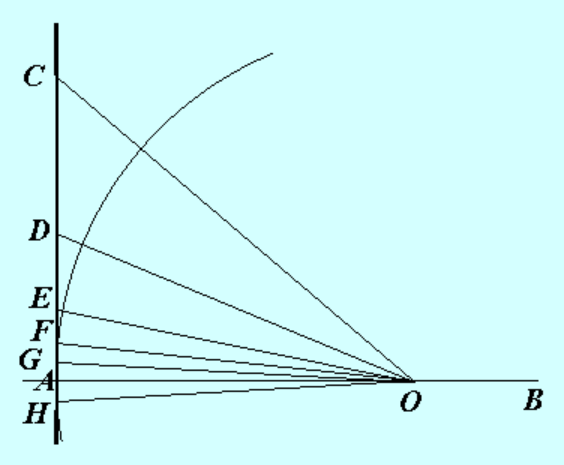
\includegraphics [scale=0.3] {pi5.png} \end{center}

$\bullet$ From above, we have that $OA : AE > 1162 \ 1/8 : 153$ and $OE : AE > 1172 \ 1/8 : 153$.

$\bullet$   $OA : AF > 2334\ 1/4 : 153$

This calculation invokes the angle bisector corollary again.

\[ \frac{OA}{FA} =  \frac{OE}{EA} + \frac{OA}{EA} \]
\[ 1162 \ 1/8 : 153 + 1172 \ 1/8 : 153 \]
which adds to give the result above.

$\bullet$  $OF : FA > 2339 \ 1/4 : 153$

Use the Pythagorean theorem to write:
\[ \frac{OF^2}{FA^2} = \frac{OA^2}{FA^2} + 1 \]
We have $(2334 \ 1/4)^2$ and $153^2 = 23409$.

Write
\[ 2334^2 + 2334/2 + 153^2 = 5447556 + 1167 +  23409 \]
\[ = 5472132  + 1/16  \]
The square root is $2339 \ 1/4$.

\subsection*{Part A, round 4}

Now draw the angle bisector $OG$.

\begin{center} 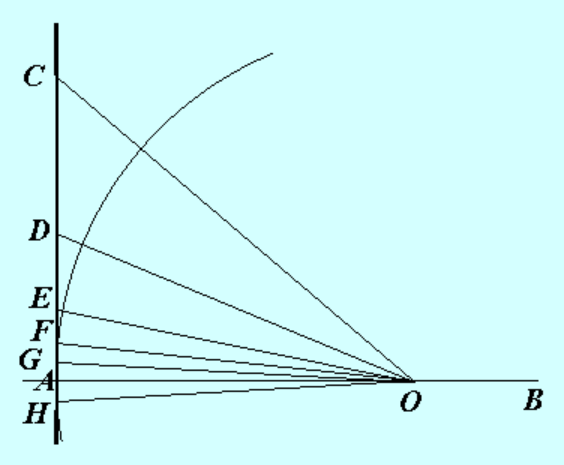
\includegraphics [scale=0.3] {pi5.png} \end{center}

$\bullet$ From above, we have that $OA : FA > 2334\ 1/4 : 153$ and $OF : FA > 2339 1/4 : 153$

Add

$\bullet$   $OA : AG > 4673\ 1/2 : 153$

We're almost done.  The original distance $AC$ was $1/12$ the perimeter of a circumscribed polygon, so we would multiply by $12$ to get the ratio to the radius, but we want the ratio to the diameter so that gives a factor of $2$ on the bottom for a total factor of $6$.  

There is an additional factor for the four "halvings" of $2^4 = 16$.  Hence we obtain

\[ 153 \times 96 = 14688 \]
and then invert to get the ratio of the circumference to the diameter:

\[ \frac{14688}{4673 \ 1/2} = 3 + \frac{668 \ 1/2}{4673 \ 1/2}  \]
The fraction is just less than $1/7$.

$1/7 = 0.142857$, while $668 \ 1/2 / 4673 \ 1/2 = 0.14304$.

We conclude that $\pi < 3 \ 1/7$.

\subsection*{Part B}

For Part B we use this diagram for an inscribed polygon.
\begin{center} 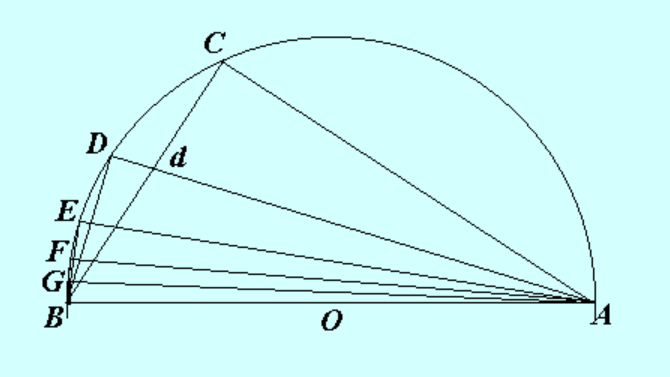
\includegraphics [scale=0.4] {pi7.png} \end{center}

As before $\triangle ABC$ is a $30-60-90$ right triangle.

$\bullet$  $AC : BC < 1351 : 780$.

This ratio is an approximation for $\sqrt{3}$.  It is an even better approximation than the previous one, and also, crucially, it is just slightly \emph{more} than the true value, whereas $265/153$ was slightly less.

\subsection*{Part B, round 1}

Let $AD$ bisect the angle, and then join $BD$.

$\bullet$  $\angle BAD = \angle dAC = \angle dBD$.
\begin{center} 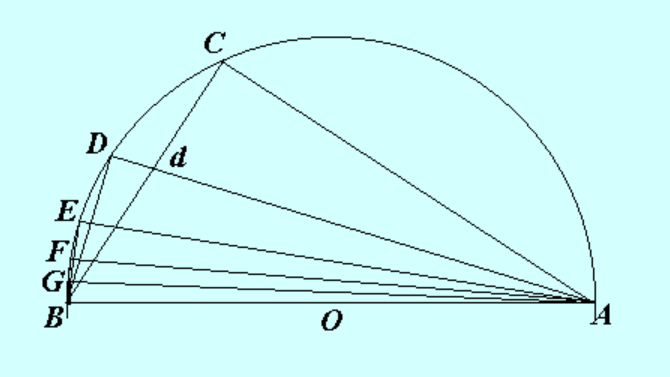
\includegraphics [scale=0.3] {pi7.png} \end{center}
The first statement just restates the construction as an angle bisector.  The second follows from the fact that the two angles have vertices on the circle and cut off the same arc.  

As a consequence, $\triangle dBD \sim \triangle dAC$.

$\bullet$  $AD : DB < 2911 : 780$

Start with the similar triangles above and write three ratios of long side (not hypotenuse) to short side
\[ AD : BD = BD : Dd = AC : Cd \]
Note: the source has $AB:Bd$ but this seems to be an error.  That is a ratio of two hypotenuses and so is not equal to the others.  As a result, I was unable to follow this part of the proof:
\begin{center} 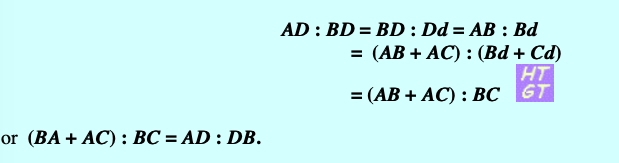
\includegraphics [scale=0.6] {pi8.png} \end{center}

However, I was able to prove the last statement
\[ (AB + AC):BC = AD:DB \]

The proof is as follows.
\begin{center} 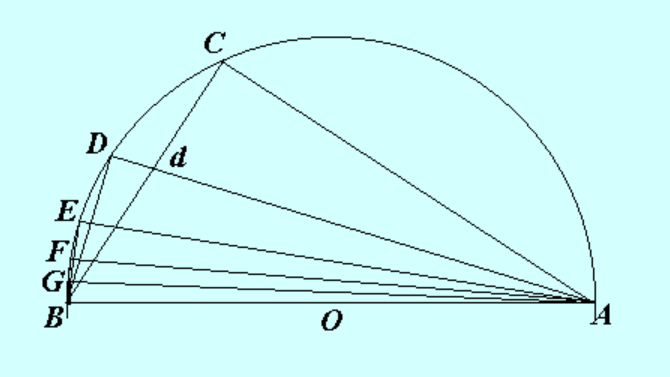
\includegraphics [scale=0.4] {pi7.png} \end{center}
We have that $\triangle ABC$ is a right triangle and that $AD$ and thus $Ad$ is the angle bisector for $\angle BAC$.  Therefore, we have by our favorite theorem that
\[ (AB + AC):BC =  AC:Cd \]
We also have that $\triangle ABD$ is a right triangle and by virtue of the angle bisector construction, $\triangle ABD$ is similar to $\triangle ACd$.  Therefore:
\[ AC:Cd = AD:DB \]
These two lines combine to give the desired result.  

The ratio $AD:DB$ is what we need going forward, and we get that from the other part:  $(AB + AC):BC$.  We have that the cotangent $AC : BC < 1351 : 780$, and $AB:BC$ is the cosecant whose value is $2$ so we multiply $780 \times 2 = 1560$, and then add $1351$ to get the numerator of the result listed above.

$\bullet$  $AB : BD < 3013 \ 3/4 : 780$

From the Pythagorean theorem:  $AD^2 + BD^2 = AB^2$ so
\[ AB^2:BD^2 = AD^2:BD^2 + 1 \]
$AD : DB < 2911 : 780$  So we obtain $2911^2 = 8473921$ and $BD^2 = 608400$ so we have that
\[ AB^2:BD^2 =  9082321: 608400 \]
\[ AB:BD <  3013 \ 3/4: 780 \]

\subsection*{Part B, round 1 summary}
Let's summarize what we did in round 1.  We started with the cosecant and the cotangent for $\triangle ABC$, namely $AB:BC$ and $:AC:BC$.

We used the relationship $(AB + AC):BC = AD:DB$ to obtain the cotangent of the bisected angle, and then we used the Pythagorean theorem in this form
\[ AB^2:BD^2 = AD^2:BD^2 + 1 \]
to get the cosecant from the cotangent.  Thus we have

$\bullet$  $AD : DB < 2911 : 780$, the cotangent.

$\bullet$  $AB : BD < 3013 \ 3/4 : 780$, the cosecant.

\subsection*{Part B, round 2}

Now, let $AE$ bisect the angle, and then join $BE$.

Rather than go through the geometry again, let's just substitute letters.  First the cotangent

\[ (AB + AD):BD = AE:EB \]

Then the cosecant.

\[ AB^2:BE^2 = AE^2:BE^2 + 1 \]

For the first part we have $2911:780 + 3013 \ 3/4:780 = 5924 \ 3/4:780$.  

We reduce the denominator to $240$.  This amounts to dividing by $3 \ 1/4$.  $5924 \ 3/4$ divided by $3 \ 1/4$ is exactly equal to $1823$.

$\bullet$ $AE:EB = 1823:240$, the cotangent.

For the second part we have the previous number squared and added to 1 and then take the square root.
$1823^2 = 3323329;  240^2 = 57600$;  so we have $3380929$ and the square root is $< 1838 \ 3/4$, but the source gives the fraction as a bit larger $1838 \ 9/11$.

$\bullet$ $AB:BE = 1838 \ 9/11: 240$, the cosecant.

\subsection*{Part B, round 3}

Now, let $AF$ bisect the angle, and then join $BF$.  Substitute letters (carefully, looking at the diagram).  First the cotangent

\[ (AB + AE):BE = AF:FB \]

Then the cosecant.

\[ AB^2:BF^2 = AF^2:BF^2 + 1 \]

For the first part we have $1838 \ 9/11: 240 + AE:EB = 1823:240 = 3661 \ 9/11:240$. 

 We reduce the denominator, this time to $66$.  This amounts to multiplication by $11/40$.  So the numerator is multiplied by the same factor giving

$\bullet$ $AF:FB = 1007:66$, the cotangent.

For the second part we have the previous number squared and added to 1 and then take the square root.$1007^2 = 1014049;  66^2 = 4356$, so we have $1018405$ and the square root is $1009 \ 1/6$.

$\bullet$ $AB:FB = 1009 \ 1/6:66$, the cosecant.

\subsection*{Part B, round 4}

Finally, let $AG$ bisect the angle, and then join $BG$.  Substitute letters.  First the cotangent

\[ (AB + AF):BF = AG:GB \]

Then the cosecant.

\[ AB^2:BG^2 = AG^2:BG^2 + 1 \]

For the first part we have

$\bullet$ $AG:GB = 2016 \ 1/6:66$, the cotangent.

Now do $2016^2 = 4064256;  66^2 = 4356$ so that's $4068612$ and the square root is $2017 \ 1/12$ while the source gives

$\bullet$ $AB:GB < 2017 \ 1/4:66$, the cosecant.

Almost done.  The side $BG$ is a side of an inscribed regular polygon of $96$ sides.  We multiply $66 \times 96 = 6336$ and compute the ratio of the inverse.  

I am not sure how Archimedes came up with it, but it is easy to verify that the ratio which is less than $\pi$ is greater than:

\[ \frac{6336}{2017 \ 1/4} > 3 \ 10/71 \]

We combine parts A and B to make our final statement that
\[ 3 \ 10/71 < \pi < 3 \ 1/7 \]


\end{document}